% Created by tikzDevice version 0.12.6 on 2025-02-15 03:35:03
% !TEX encoding = UTF-8 Unicode
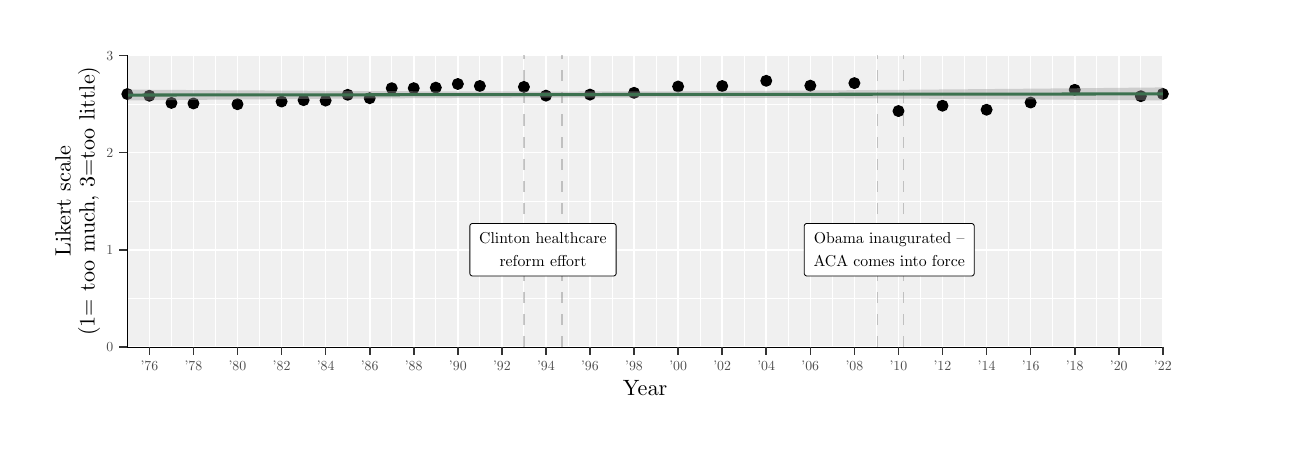
\begin{tikzpicture}[x=1pt,y=1pt]
\definecolor{fillColor}{RGB}{255,255,255}
\path[use as bounding box,fill=fillColor,fill opacity=0.00] (0,0) rectangle (455.30,144.54);
\begin{scope}
\path[clip] (  0.00,  0.00) rectangle (455.30,144.54);
\definecolor{drawColor}{RGB}{255,255,255}
\definecolor{fillColor}{RGB}{255,255,255}

\path[draw=drawColor,line width= 0.6pt,line join=round,line cap=round,fill=fillColor] ( -0.00,  0.00) rectangle (455.30,144.54);
\end{scope}
\begin{scope}
\path[clip] (  0.00,  0.00) rectangle (455.30,144.54);
\definecolor{fillColor}{gray}{0.94}

\path[fill=fillColor] ( 35.90, 29.18) rectangle (410.30,134.54);
\definecolor{drawColor}{RGB}{255,255,255}

\path[draw=drawColor,line width= 0.3pt,line join=round] ( 35.90, 46.74) --
	(410.30, 46.74);

\path[draw=drawColor,line width= 0.3pt,line join=round] ( 35.90, 81.86) --
	(410.30, 81.86);

\path[draw=drawColor,line width= 0.3pt,line join=round] ( 35.90,116.98) --
	(410.30,116.98);

\path[draw=drawColor,line width= 0.3pt,line join=round] ( 36.01, 29.18) --
	( 36.01,134.54);

\path[draw=drawColor,line width= 0.3pt,line join=round] ( 51.94, 29.18) --
	( 51.94,134.54);

\path[draw=drawColor,line width= 0.3pt,line join=round] ( 67.86, 29.18) --
	( 67.86,134.54);

\path[draw=drawColor,line width= 0.3pt,line join=round] ( 83.78, 29.18) --
	( 83.78,134.54);

\path[draw=drawColor,line width= 0.3pt,line join=round] ( 99.70, 29.18) --
	( 99.70,134.54);

\path[draw=drawColor,line width= 0.3pt,line join=round] (115.62, 29.18) --
	(115.62,134.54);

\path[draw=drawColor,line width= 0.3pt,line join=round] (131.55, 29.18) --
	(131.55,134.54);

\path[draw=drawColor,line width= 0.3pt,line join=round] (147.47, 29.18) --
	(147.47,134.54);

\path[draw=drawColor,line width= 0.3pt,line join=round] (163.39, 29.18) --
	(163.39,134.54);

\path[draw=drawColor,line width= 0.3pt,line join=round] (179.31, 29.18) --
	(179.31,134.54);

\path[draw=drawColor,line width= 0.3pt,line join=round] (195.24, 29.18) --
	(195.24,134.54);

\path[draw=drawColor,line width= 0.3pt,line join=round] (211.16, 29.18) --
	(211.16,134.54);

\path[draw=drawColor,line width= 0.3pt,line join=round] (227.08, 29.18) --
	(227.08,134.54);

\path[draw=drawColor,line width= 0.3pt,line join=round] (243.00, 29.18) --
	(243.00,134.54);

\path[draw=drawColor,line width= 0.3pt,line join=round] (258.93, 29.18) --
	(258.93,134.54);

\path[draw=drawColor,line width= 0.3pt,line join=round] (274.85, 29.18) --
	(274.85,134.54);

\path[draw=drawColor,line width= 0.3pt,line join=round] (290.77, 29.18) --
	(290.77,134.54);

\path[draw=drawColor,line width= 0.3pt,line join=round] (306.69, 29.18) --
	(306.69,134.54);

\path[draw=drawColor,line width= 0.3pt,line join=round] (322.61, 29.18) --
	(322.61,134.54);

\path[draw=drawColor,line width= 0.3pt,line join=round] (338.54, 29.18) --
	(338.54,134.54);

\path[draw=drawColor,line width= 0.3pt,line join=round] (354.46, 29.18) --
	(354.46,134.54);

\path[draw=drawColor,line width= 0.3pt,line join=round] (370.38, 29.18) --
	(370.38,134.54);

\path[draw=drawColor,line width= 0.3pt,line join=round] (386.30, 29.18) --
	(386.30,134.54);

\path[draw=drawColor,line width= 0.3pt,line join=round] (402.23, 29.18) --
	(402.23,134.54);

\path[draw=drawColor,line width= 0.6pt,line join=round] ( 35.90, 29.18) --
	(410.30, 29.18);

\path[draw=drawColor,line width= 0.6pt,line join=round] ( 35.90, 64.30) --
	(410.30, 64.30);

\path[draw=drawColor,line width= 0.6pt,line join=round] ( 35.90, 99.42) --
	(410.30, 99.42);

\path[draw=drawColor,line width= 0.6pt,line join=round] ( 35.90,134.54) --
	(410.30,134.54);

\path[draw=drawColor,line width= 0.6pt,line join=round] ( 43.97, 29.18) --
	( 43.97,134.54);

\path[draw=drawColor,line width= 0.6pt,line join=round] ( 59.90, 29.18) --
	( 59.90,134.54);

\path[draw=drawColor,line width= 0.6pt,line join=round] ( 75.81, 29.18) --
	( 75.81,134.54);

\path[draw=drawColor,line width= 0.6pt,line join=round] ( 91.75, 29.18) --
	( 91.75,134.54);

\path[draw=drawColor,line width= 0.6pt,line join=round] (107.66, 29.18) --
	(107.66,134.54);

\path[draw=drawColor,line width= 0.6pt,line join=round] (123.59, 29.18) --
	(123.59,134.54);

\path[draw=drawColor,line width= 0.6pt,line join=round] (139.50, 29.18) --
	(139.50,134.54);

\path[draw=drawColor,line width= 0.6pt,line join=round] (155.44, 29.18) --
	(155.44,134.54);

\path[draw=drawColor,line width= 0.6pt,line join=round] (171.35, 29.18) --
	(171.35,134.54);

\path[draw=drawColor,line width= 0.6pt,line join=round] (187.28, 29.18) --
	(187.28,134.54);

\path[draw=drawColor,line width= 0.6pt,line join=round] (203.19, 29.18) --
	(203.19,134.54);

\path[draw=drawColor,line width= 0.6pt,line join=round] (219.12, 29.18) --
	(219.12,134.54);

\path[draw=drawColor,line width= 0.6pt,line join=round] (235.04, 29.18) --
	(235.04,134.54);

\path[draw=drawColor,line width= 0.6pt,line join=round] (250.97, 29.18) --
	(250.97,134.54);

\path[draw=drawColor,line width= 0.6pt,line join=round] (266.88, 29.18) --
	(266.88,134.54);

\path[draw=drawColor,line width= 0.6pt,line join=round] (282.81, 29.18) --
	(282.81,134.54);

\path[draw=drawColor,line width= 0.6pt,line join=round] (298.73, 29.18) --
	(298.73,134.54);

\path[draw=drawColor,line width= 0.6pt,line join=round] (314.66, 29.18) --
	(314.66,134.54);

\path[draw=drawColor,line width= 0.6pt,line join=round] (330.57, 29.18) --
	(330.57,134.54);

\path[draw=drawColor,line width= 0.6pt,line join=round] (346.50, 29.18) --
	(346.50,134.54);

\path[draw=drawColor,line width= 0.6pt,line join=round] (362.41, 29.18) --
	(362.41,134.54);

\path[draw=drawColor,line width= 0.6pt,line join=round] (378.35, 29.18) --
	(378.35,134.54);

\path[draw=drawColor,line width= 0.6pt,line join=round] (394.26, 29.18) --
	(394.26,134.54);

\path[draw=drawColor,line width= 0.6pt,line join=round] (410.19, 29.18) --
	(410.19,134.54);
\definecolor{drawColor}{RGB}{0,0,0}

\path[draw=drawColor,draw opacity=0.20,line width= 0.6pt,dash pattern=on 4pt off 4pt ,line join=round] (179.32, 29.18) -- (179.32,134.54);

\path[draw=drawColor,draw opacity=0.20,line width= 0.6pt,dash pattern=on 4pt off 4pt ,line join=round] (193.12, 29.18) -- (193.12,134.54);

\path[draw=drawColor,draw opacity=0.20,line width= 0.6pt,dash pattern=on 4pt off 4pt ,line join=round] (307.12, 29.18) -- (307.12,134.54);

\path[draw=drawColor,draw opacity=0.20,line width= 0.6pt,dash pattern=on 4pt off 4pt ,line join=round] (316.42, 29.18) -- (316.42,134.54);
\definecolor{drawColor}{RGB}{0,0,0}
\definecolor{fillColor}{RGB}{0,0,0}

\path[draw=drawColor,line width= 0.4pt,line join=round,line cap=round,fill=fillColor] ( 36.01,120.55) circle (  1.96);

\path[draw=drawColor,line width= 0.4pt,line join=round,line cap=round,fill=fillColor] ( 43.97,119.94) circle (  1.96);

\path[draw=drawColor,line width= 0.4pt,line join=round,line cap=round,fill=fillColor] ( 51.95,117.35) circle (  1.96);

\path[draw=drawColor,line width= 0.4pt,line join=round,line cap=round,fill=fillColor] ( 59.90,117.16) circle (  1.96);

\path[draw=drawColor,line width= 0.4pt,line join=round,line cap=round,fill=fillColor] ( 75.81,116.87) circle (  1.96);

\path[draw=drawColor,line width= 0.4pt,line join=round,line cap=round,fill=fillColor] ( 91.75,117.85) circle (  1.96);

\path[draw=drawColor,line width= 0.4pt,line join=round,line cap=round,fill=fillColor] ( 99.70,118.35) circle (  1.96);

\path[draw=drawColor,line width= 0.4pt,line join=round,line cap=round,fill=fillColor] (107.66,118.19) circle (  1.96);

\path[draw=drawColor,line width= 0.4pt,line join=round,line cap=round,fill=fillColor] (115.64,120.28) circle (  1.96);

\path[draw=drawColor,line width= 0.4pt,line join=round,line cap=round,fill=fillColor] (123.59,119.06) circle (  1.96);

\path[draw=drawColor,line width= 0.4pt,line join=round,line cap=round,fill=fillColor] (131.55,122.67) circle (  1.96);

\path[draw=drawColor,line width= 0.4pt,line join=round,line cap=round,fill=fillColor] (139.50,122.68) circle (  1.96);

\path[draw=drawColor,line width= 0.4pt,line join=round,line cap=round,fill=fillColor] (147.48,122.87) circle (  1.96);

\path[draw=drawColor,line width= 0.4pt,line join=round,line cap=round,fill=fillColor] (155.44,124.19) circle (  1.96);

\path[draw=drawColor,line width= 0.4pt,line join=round,line cap=round,fill=fillColor] (163.39,123.47) circle (  1.96);

\path[draw=drawColor,line width= 0.4pt,line join=round,line cap=round,fill=fillColor] (179.32,123.13) circle (  1.96);

\path[draw=drawColor,line width= 0.4pt,line join=round,line cap=round,fill=fillColor] (187.28,119.97) circle (  1.96);

\path[draw=drawColor,line width= 0.4pt,line join=round,line cap=round,fill=fillColor] (203.19,120.35) circle (  1.96);

\path[draw=drawColor,line width= 0.4pt,line join=round,line cap=round,fill=fillColor] (219.12,121.00) circle (  1.96);

\path[draw=drawColor,line width= 0.4pt,line join=round,line cap=round,fill=fillColor] (235.04,123.28) circle (  1.96);

\path[draw=drawColor,line width= 0.4pt,line join=round,line cap=round,fill=fillColor] (250.97,123.45) circle (  1.96);

\path[draw=drawColor,line width= 0.4pt,line join=round,line cap=round,fill=fillColor] (266.88,125.34) circle (  1.96);

\path[draw=drawColor,line width= 0.4pt,line join=round,line cap=round,fill=fillColor] (282.81,123.58) circle (  1.96);

\path[draw=drawColor,line width= 0.4pt,line join=round,line cap=round,fill=fillColor] (298.73,124.50) circle (  1.96);

\path[draw=drawColor,line width= 0.4pt,line join=round,line cap=round,fill=fillColor] (314.66,114.41) circle (  1.96);

\path[draw=drawColor,line width= 0.4pt,line join=round,line cap=round,fill=fillColor] (330.57,116.34) circle (  1.96);

\path[draw=drawColor,line width= 0.4pt,line join=round,line cap=round,fill=fillColor] (346.50,114.88) circle (  1.96);

\path[draw=drawColor,line width= 0.4pt,line join=round,line cap=round,fill=fillColor] (362.41,117.49) circle (  1.96);

\path[draw=drawColor,line width= 0.4pt,line join=round,line cap=round,fill=fillColor] (378.35,122.08) circle (  1.96);

\path[draw=drawColor,line width= 0.4pt,line join=round,line cap=round,fill=fillColor] (402.24,119.78) circle (  1.96);

\path[draw=drawColor,line width= 0.4pt,line join=round,line cap=round,fill=fillColor] (410.19,120.60) circle (  1.96);
\definecolor{fillColor}{RGB}{153,153,153}

\path[fill=fillColor,fill opacity=0.40] ( 36.01,122.16) --
	( 40.75,122.13) --
	( 45.49,122.09) --
	( 50.22,122.06) --
	( 54.96,122.03) --
	( 59.70,122.00) --
	( 64.43,121.97) --
	( 69.17,121.93) --
	( 73.90,121.90) --
	( 78.64,121.87) --
	( 83.38,121.85) --
	( 88.11,121.82) --
	( 92.85,121.79) --
	( 97.59,121.76) --
	(102.32,121.74) --
	(107.06,121.71) --
	(111.80,121.69) --
	(116.53,121.66) --
	(121.27,121.64) --
	(126.01,121.62) --
	(130.74,121.60) --
	(135.48,121.58) --
	(140.21,121.56) --
	(144.95,121.55) --
	(149.69,121.53) --
	(154.42,121.52) --
	(159.16,121.51) --
	(163.90,121.50) --
	(168.63,121.49) --
	(173.37,121.48) --
	(178.11,121.48) --
	(182.84,121.47) --
	(187.58,121.47) --
	(192.32,121.47) --
	(197.05,121.47) --
	(201.79,121.48) --
	(206.53,121.49) --
	(211.26,121.50) --
	(216.00,121.51) --
	(220.73,121.52) --
	(225.47,121.53) --
	(230.21,121.55) --
	(234.94,121.57) --
	(239.68,121.59) --
	(244.42,121.61) --
	(249.15,121.63) --
	(253.89,121.66) --
	(258.63,121.68) --
	(263.36,121.71) --
	(268.10,121.74) --
	(272.84,121.77) --
	(277.57,121.80) --
	(282.31,121.83) --
	(287.04,121.86) --
	(291.78,121.90) --
	(296.52,121.93) --
	(301.25,121.97) --
	(305.99,122.01) --
	(310.73,122.04) --
	(315.46,122.08) --
	(320.20,122.12) --
	(324.94,122.16) --
	(329.67,122.20) --
	(334.41,122.24) --
	(339.15,122.28) --
	(343.88,122.33) --
	(348.62,122.37) --
	(353.35,122.41) --
	(358.09,122.45) --
	(362.83,122.50) --
	(367.56,122.54) --
	(372.30,122.58) --
	(377.04,122.63) --
	(381.77,122.67) --
	(386.51,122.72) --
	(391.25,122.76) --
	(395.98,122.81) --
	(400.72,122.86) --
	(405.46,122.90) --
	(410.19,122.95) --
	(410.19,118.26) --
	(405.46,118.29) --
	(400.72,118.33) --
	(395.98,118.36) --
	(391.25,118.40) --
	(386.51,118.43) --
	(381.77,118.47) --
	(377.04,118.50) --
	(372.30,118.54) --
	(367.56,118.57) --
	(362.83,118.61) --
	(358.09,118.64) --
	(353.35,118.67) --
	(348.62,118.70) --
	(343.88,118.74) --
	(339.15,118.77) --
	(334.41,118.80) --
	(329.67,118.83) --
	(324.94,118.86) --
	(320.20,118.89) --
	(315.46,118.92) --
	(310.73,118.95) --
	(305.99,118.97) --
	(301.25,119.00) --
	(296.52,119.03) --
	(291.78,119.05) --
	(287.04,119.07) --
	(282.31,119.10) --
	(277.57,119.12) --
	(272.84,119.14) --
	(268.10,119.16) --
	(263.36,119.18) --
	(258.63,119.20) --
	(253.89,119.21) --
	(249.15,119.23) --
	(244.42,119.24) --
	(239.68,119.25) --
	(234.94,119.26) --
	(230.21,119.27) --
	(225.47,119.27) --
	(220.73,119.28) --
	(216.00,119.28) --
	(211.26,119.28) --
	(206.53,119.28) --
	(201.79,119.28) --
	(197.05,119.27) --
	(192.32,119.26) --
	(187.58,119.25) --
	(182.84,119.24) --
	(178.11,119.23) --
	(173.37,119.21) --
	(168.63,119.20) --
	(163.90,119.18) --
	(159.16,119.16) --
	(154.42,119.13) --
	(149.69,119.11) --
	(144.95,119.09) --
	(140.21,119.06) --
	(135.48,119.03) --
	(130.74,119.00) --
	(126.01,118.97) --
	(121.27,118.94) --
	(116.53,118.91) --
	(111.80,118.87) --
	(107.06,118.84) --
	(102.32,118.80) --
	( 97.59,118.77) --
	( 92.85,118.73) --
	( 88.11,118.69) --
	( 83.38,118.65) --
	( 78.64,118.61) --
	( 73.90,118.57) --
	( 69.17,118.53) --
	( 64.43,118.49) --
	( 59.70,118.45) --
	( 54.96,118.41) --
	( 50.22,118.37) --
	( 45.49,118.32) --
	( 40.75,118.28) --
	( 36.01,118.24) --
	cycle;

\path[] ( 36.01,122.16) --
	( 40.75,122.13) --
	( 45.49,122.09) --
	( 50.22,122.06) --
	( 54.96,122.03) --
	( 59.70,122.00) --
	( 64.43,121.97) --
	( 69.17,121.93) --
	( 73.90,121.90) --
	( 78.64,121.87) --
	( 83.38,121.85) --
	( 88.11,121.82) --
	( 92.85,121.79) --
	( 97.59,121.76) --
	(102.32,121.74) --
	(107.06,121.71) --
	(111.80,121.69) --
	(116.53,121.66) --
	(121.27,121.64) --
	(126.01,121.62) --
	(130.74,121.60) --
	(135.48,121.58) --
	(140.21,121.56) --
	(144.95,121.55) --
	(149.69,121.53) --
	(154.42,121.52) --
	(159.16,121.51) --
	(163.90,121.50) --
	(168.63,121.49) --
	(173.37,121.48) --
	(178.11,121.48) --
	(182.84,121.47) --
	(187.58,121.47) --
	(192.32,121.47) --
	(197.05,121.47) --
	(201.79,121.48) --
	(206.53,121.49) --
	(211.26,121.50) --
	(216.00,121.51) --
	(220.73,121.52) --
	(225.47,121.53) --
	(230.21,121.55) --
	(234.94,121.57) --
	(239.68,121.59) --
	(244.42,121.61) --
	(249.15,121.63) --
	(253.89,121.66) --
	(258.63,121.68) --
	(263.36,121.71) --
	(268.10,121.74) --
	(272.84,121.77) --
	(277.57,121.80) --
	(282.31,121.83) --
	(287.04,121.86) --
	(291.78,121.90) --
	(296.52,121.93) --
	(301.25,121.97) --
	(305.99,122.01) --
	(310.73,122.04) --
	(315.46,122.08) --
	(320.20,122.12) --
	(324.94,122.16) --
	(329.67,122.20) --
	(334.41,122.24) --
	(339.15,122.28) --
	(343.88,122.33) --
	(348.62,122.37) --
	(353.35,122.41) --
	(358.09,122.45) --
	(362.83,122.50) --
	(367.56,122.54) --
	(372.30,122.58) --
	(377.04,122.63) --
	(381.77,122.67) --
	(386.51,122.72) --
	(391.25,122.76) --
	(395.98,122.81) --
	(400.72,122.86) --
	(405.46,122.90) --
	(410.19,122.95);

\path[] (410.19,118.26) --
	(405.46,118.29) --
	(400.72,118.33) --
	(395.98,118.36) --
	(391.25,118.40) --
	(386.51,118.43) --
	(381.77,118.47) --
	(377.04,118.50) --
	(372.30,118.54) --
	(367.56,118.57) --
	(362.83,118.61) --
	(358.09,118.64) --
	(353.35,118.67) --
	(348.62,118.70) --
	(343.88,118.74) --
	(339.15,118.77) --
	(334.41,118.80) --
	(329.67,118.83) --
	(324.94,118.86) --
	(320.20,118.89) --
	(315.46,118.92) --
	(310.73,118.95) --
	(305.99,118.97) --
	(301.25,119.00) --
	(296.52,119.03) --
	(291.78,119.05) --
	(287.04,119.07) --
	(282.31,119.10) --
	(277.57,119.12) --
	(272.84,119.14) --
	(268.10,119.16) --
	(263.36,119.18) --
	(258.63,119.20) --
	(253.89,119.21) --
	(249.15,119.23) --
	(244.42,119.24) --
	(239.68,119.25) --
	(234.94,119.26) --
	(230.21,119.27) --
	(225.47,119.27) --
	(220.73,119.28) --
	(216.00,119.28) --
	(211.26,119.28) --
	(206.53,119.28) --
	(201.79,119.28) --
	(197.05,119.27) --
	(192.32,119.26) --
	(187.58,119.25) --
	(182.84,119.24) --
	(178.11,119.23) --
	(173.37,119.21) --
	(168.63,119.20) --
	(163.90,119.18) --
	(159.16,119.16) --
	(154.42,119.13) --
	(149.69,119.11) --
	(144.95,119.09) --
	(140.21,119.06) --
	(135.48,119.03) --
	(130.74,119.00) --
	(126.01,118.97) --
	(121.27,118.94) --
	(116.53,118.91) --
	(111.80,118.87) --
	(107.06,118.84) --
	(102.32,118.80) --
	( 97.59,118.77) --
	( 92.85,118.73) --
	( 88.11,118.69) --
	( 83.38,118.65) --
	( 78.64,118.61) --
	( 73.90,118.57) --
	( 69.17,118.53) --
	( 64.43,118.49) --
	( 59.70,118.45) --
	( 54.96,118.41) --
	( 50.22,118.37) --
	( 45.49,118.32) --
	( 40.75,118.28) --
	( 36.01,118.24);
\definecolor{drawColor}{RGB}{60,113,79}

\path[draw=drawColor,line width= 1.1pt,line join=round] ( 36.01,120.20) --
	( 40.75,120.20) --
	( 45.49,120.21) --
	( 50.22,120.21) --
	( 54.96,120.22) --
	( 59.70,120.22) --
	( 64.43,120.23) --
	( 69.17,120.23) --
	( 73.90,120.24) --
	( 78.64,120.24) --
	( 83.38,120.25) --
	( 88.11,120.25) --
	( 92.85,120.26) --
	( 97.59,120.26) --
	(102.32,120.27) --
	(107.06,120.28) --
	(111.80,120.28) --
	(116.53,120.29) --
	(121.27,120.29) --
	(126.01,120.30) --
	(130.74,120.30) --
	(135.48,120.31) --
	(140.21,120.31) --
	(144.95,120.32) --
	(149.69,120.32) --
	(154.42,120.33) --
	(159.16,120.33) --
	(163.90,120.34) --
	(168.63,120.34) --
	(173.37,120.35) --
	(178.11,120.35) --
	(182.84,120.36) --
	(187.58,120.36) --
	(192.32,120.37) --
	(197.05,120.37) --
	(201.79,120.38) --
	(206.53,120.38) --
	(211.26,120.39) --
	(216.00,120.39) --
	(220.73,120.40) --
	(225.47,120.40) --
	(230.21,120.41) --
	(234.94,120.41) --
	(239.68,120.42) --
	(244.42,120.42) --
	(249.15,120.43) --
	(253.89,120.43) --
	(258.63,120.44) --
	(263.36,120.44) --
	(268.10,120.45) --
	(272.84,120.45) --
	(277.57,120.46) --
	(282.31,120.46) --
	(287.04,120.47) --
	(291.78,120.47) --
	(296.52,120.48) --
	(301.25,120.48) --
	(305.99,120.49) --
	(310.73,120.50) --
	(315.46,120.50) --
	(320.20,120.51) --
	(324.94,120.51) --
	(329.67,120.52) --
	(334.41,120.52) --
	(339.15,120.53) --
	(343.88,120.53) --
	(348.62,120.54) --
	(353.35,120.54) --
	(358.09,120.55) --
	(362.83,120.55) --
	(367.56,120.56) --
	(372.30,120.56) --
	(377.04,120.57) --
	(381.77,120.57) --
	(386.51,120.58) --
	(391.25,120.58) --
	(395.98,120.59) --
	(400.72,120.59) --
	(405.46,120.60) --
	(410.19,120.60);
\definecolor{drawColor}{RGB}{0,0,0}
\definecolor{fillColor}{RGB}{255,255,255}

\path[draw=drawColor,line width= 0.3pt,line join=round,line cap=round,fill=fillColor] (160.81, 54.82) --
	(211.61, 54.82) --
	(211.57, 54.82) --
	(211.74, 54.82) --
	(211.90, 54.86) --
	(212.06, 54.92) --
	(212.20, 55.00) --
	(212.33, 55.10) --
	(212.44, 55.23) --
	(212.53, 55.37) --
	(212.59, 55.52) --
	(212.63, 55.68) --
	(212.64, 55.84) --
	(212.64, 55.84) --
	(212.64, 72.76) --
	(212.64, 72.76) --
	(212.63, 72.92) --
	(212.59, 73.08) --
	(212.53, 73.23) --
	(212.44, 73.37) --
	(212.33, 73.50) --
	(212.20, 73.60) --
	(212.06, 73.69) --
	(211.90, 73.74) --
	(211.74, 73.78) --
	(211.61, 73.78) --
	(160.81, 73.78) --
	(160.93, 73.78) --
	(160.77, 73.78) --
	(160.60, 73.76) --
	(160.45, 73.72) --
	(160.30, 73.65) --
	(160.16, 73.55) --
	(160.04, 73.44) --
	(159.94, 73.31) --
	(159.86, 73.16) --
	(159.81, 73.00) --
	(159.78, 72.84) --
	(159.78, 72.76) --
	(159.78, 55.84) --
	(159.78, 55.93) --
	(159.78, 55.76) --
	(159.81, 55.60) --
	(159.86, 55.44) --
	(159.94, 55.29) --
	(160.04, 55.16) --
	(160.16, 55.05) --
	(160.30, 54.95) --
	(160.45, 54.88) --
	(160.60, 54.84) --
	(160.77, 54.82) --
	cycle;
\end{scope}
\begin{scope}
\path[clip] (  0.00,  0.00) rectangle (455.30,144.54);
\definecolor{drawColor}{RGB}{0,0,0}

\node[text=drawColor,anchor=base,inner sep=0pt, outer sep=0pt, scale=  0.57] at (186.21, 66.44) {Clinton healthcare };

\node[text=drawColor,anchor=base,inner sep=0pt, outer sep=0pt, scale=  0.57] at (186.21, 58.24) { reform effort};
\end{scope}
\begin{scope}
\path[clip] (  0.00,  0.00) rectangle (455.30,144.54);
\definecolor{drawColor}{RGB}{0,0,0}
\definecolor{fillColor}{RGB}{255,255,255}

\path[draw=drawColor,line width= 0.3pt,line join=round,line cap=round,fill=fillColor] (281.64, 54.82) --
	(341.01, 54.82) --
	(340.97, 54.82) --
	(341.13, 54.82) --
	(341.30, 54.86) --
	(341.45, 54.92) --
	(341.59, 55.00) --
	(341.72, 55.10) --
	(341.83, 55.23) --
	(341.92, 55.37) --
	(341.98, 55.52) --
	(342.02, 55.68) --
	(342.04, 55.84) --
	(342.04, 55.84) --
	(342.04, 72.76) --
	(342.04, 72.76) --
	(342.02, 72.92) --
	(341.98, 73.08) --
	(341.92, 73.23) --
	(341.83, 73.37) --
	(341.72, 73.50) --
	(341.59, 73.60) --
	(341.45, 73.69) --
	(341.30, 73.74) --
	(341.13, 73.78) --
	(341.01, 73.78) --
	(281.64, 73.78) --
	(281.76, 73.78) --
	(281.60, 73.78) --
	(281.43, 73.76) --
	(281.27, 73.72) --
	(281.12, 73.65) --
	(280.99, 73.55) --
	(280.87, 73.44) --
	(280.77, 73.31) --
	(280.69, 73.16) --
	(280.64, 73.00) --
	(280.61, 72.84) --
	(280.61, 72.76) --
	(280.61, 55.84) --
	(280.61, 55.93) --
	(280.61, 55.76) --
	(280.64, 55.60) --
	(280.69, 55.44) --
	(280.77, 55.29) --
	(280.87, 55.16) --
	(280.99, 55.05) --
	(281.12, 54.95) --
	(281.27, 54.88) --
	(281.43, 54.84) --
	(281.60, 54.82) --
	cycle;
\end{scope}
\begin{scope}
\path[clip] (  0.00,  0.00) rectangle (455.30,144.54);
\definecolor{drawColor}{RGB}{0,0,0}

\node[text=drawColor,anchor=base,inner sep=0pt, outer sep=0pt, scale=  0.57] at (311.32, 66.44) {Obama inaugurated -- };

\node[text=drawColor,anchor=base,inner sep=0pt, outer sep=0pt, scale=  0.57] at (311.32, 58.24) { ACA comes into force};
\end{scope}
\begin{scope}
\path[clip] (  0.00,  0.00) rectangle (455.30,144.54);
\definecolor{drawColor}{RGB}{0,0,0}

\path[draw=drawColor,line width= 0.2pt,line join=round] ( 35.90, 29.18) --
	( 35.90,134.54);
\end{scope}
\begin{scope}
\path[clip] (  0.00,  0.00) rectangle (455.30,144.54);
\definecolor{drawColor}{gray}{0.30}

\node[text=drawColor,anchor=base east,inner sep=0pt, outer sep=0pt, scale=  0.50] at ( 30.95, 27.46) {0};

\node[text=drawColor,anchor=base east,inner sep=0pt, outer sep=0pt, scale=  0.50] at ( 30.95, 62.58) {1};

\node[text=drawColor,anchor=base east,inner sep=0pt, outer sep=0pt, scale=  0.50] at ( 30.95, 97.70) {2};

\node[text=drawColor,anchor=base east,inner sep=0pt, outer sep=0pt, scale=  0.50] at ( 30.95,132.82) {3};
\end{scope}
\begin{scope}
\path[clip] (  0.00,  0.00) rectangle (455.30,144.54);
\definecolor{drawColor}{gray}{0.20}

\path[draw=drawColor,line width= 0.6pt,line join=round] ( 33.15, 29.18) --
	( 35.90, 29.18);

\path[draw=drawColor,line width= 0.6pt,line join=round] ( 33.15, 64.30) --
	( 35.90, 64.30);

\path[draw=drawColor,line width= 0.6pt,line join=round] ( 33.15, 99.42) --
	( 35.90, 99.42);

\path[draw=drawColor,line width= 0.6pt,line join=round] ( 33.15,134.54) --
	( 35.90,134.54);
\end{scope}
\begin{scope}
\path[clip] (  0.00,  0.00) rectangle (455.30,144.54);
\definecolor{drawColor}{RGB}{0,0,0}

\path[draw=drawColor,line width= 0.2pt,line join=round] ( 35.90, 29.18) --
	(410.30, 29.18);
\end{scope}
\begin{scope}
\path[clip] (  0.00,  0.00) rectangle (455.30,144.54);
\definecolor{drawColor}{gray}{0.20}

\path[draw=drawColor,line width= 0.6pt,line join=round] ( 43.97, 26.43) --
	( 43.97, 29.18);

\path[draw=drawColor,line width= 0.6pt,line join=round] ( 59.90, 26.43) --
	( 59.90, 29.18);

\path[draw=drawColor,line width= 0.6pt,line join=round] ( 75.81, 26.43) --
	( 75.81, 29.18);

\path[draw=drawColor,line width= 0.6pt,line join=round] ( 91.75, 26.43) --
	( 91.75, 29.18);

\path[draw=drawColor,line width= 0.6pt,line join=round] (107.66, 26.43) --
	(107.66, 29.18);

\path[draw=drawColor,line width= 0.6pt,line join=round] (123.59, 26.43) --
	(123.59, 29.18);

\path[draw=drawColor,line width= 0.6pt,line join=round] (139.50, 26.43) --
	(139.50, 29.18);

\path[draw=drawColor,line width= 0.6pt,line join=round] (155.44, 26.43) --
	(155.44, 29.18);

\path[draw=drawColor,line width= 0.6pt,line join=round] (171.35, 26.43) --
	(171.35, 29.18);

\path[draw=drawColor,line width= 0.6pt,line join=round] (187.28, 26.43) --
	(187.28, 29.18);

\path[draw=drawColor,line width= 0.6pt,line join=round] (203.19, 26.43) --
	(203.19, 29.18);

\path[draw=drawColor,line width= 0.6pt,line join=round] (219.12, 26.43) --
	(219.12, 29.18);

\path[draw=drawColor,line width= 0.6pt,line join=round] (235.04, 26.43) --
	(235.04, 29.18);

\path[draw=drawColor,line width= 0.6pt,line join=round] (250.97, 26.43) --
	(250.97, 29.18);

\path[draw=drawColor,line width= 0.6pt,line join=round] (266.88, 26.43) --
	(266.88, 29.18);

\path[draw=drawColor,line width= 0.6pt,line join=round] (282.81, 26.43) --
	(282.81, 29.18);

\path[draw=drawColor,line width= 0.6pt,line join=round] (298.73, 26.43) --
	(298.73, 29.18);

\path[draw=drawColor,line width= 0.6pt,line join=round] (314.66, 26.43) --
	(314.66, 29.18);

\path[draw=drawColor,line width= 0.6pt,line join=round] (330.57, 26.43) --
	(330.57, 29.18);

\path[draw=drawColor,line width= 0.6pt,line join=round] (346.50, 26.43) --
	(346.50, 29.18);

\path[draw=drawColor,line width= 0.6pt,line join=round] (362.41, 26.43) --
	(362.41, 29.18);

\path[draw=drawColor,line width= 0.6pt,line join=round] (378.35, 26.43) --
	(378.35, 29.18);

\path[draw=drawColor,line width= 0.6pt,line join=round] (394.26, 26.43) --
	(394.26, 29.18);

\path[draw=drawColor,line width= 0.6pt,line join=round] (410.19, 26.43) --
	(410.19, 29.18);
\end{scope}
\begin{scope}
\path[clip] (  0.00,  0.00) rectangle (455.30,144.54);
\definecolor{drawColor}{gray}{0.30}

\node[text=drawColor,anchor=base,inner sep=0pt, outer sep=0pt, scale=  0.50] at ( 43.97, 20.79) {'76};

\node[text=drawColor,anchor=base,inner sep=0pt, outer sep=0pt, scale=  0.50] at ( 59.90, 20.79) {'78};

\node[text=drawColor,anchor=base,inner sep=0pt, outer sep=0pt, scale=  0.50] at ( 75.81, 20.79) {'80};

\node[text=drawColor,anchor=base,inner sep=0pt, outer sep=0pt, scale=  0.50] at ( 91.75, 20.79) {'82};

\node[text=drawColor,anchor=base,inner sep=0pt, outer sep=0pt, scale=  0.50] at (107.66, 20.79) {'84};

\node[text=drawColor,anchor=base,inner sep=0pt, outer sep=0pt, scale=  0.50] at (123.59, 20.79) {'86};

\node[text=drawColor,anchor=base,inner sep=0pt, outer sep=0pt, scale=  0.50] at (139.50, 20.79) {'88};

\node[text=drawColor,anchor=base,inner sep=0pt, outer sep=0pt, scale=  0.50] at (155.44, 20.79) {'90};

\node[text=drawColor,anchor=base,inner sep=0pt, outer sep=0pt, scale=  0.50] at (171.35, 20.79) {'92};

\node[text=drawColor,anchor=base,inner sep=0pt, outer sep=0pt, scale=  0.50] at (187.28, 20.79) {'94};

\node[text=drawColor,anchor=base,inner sep=0pt, outer sep=0pt, scale=  0.50] at (203.19, 20.79) {'96};

\node[text=drawColor,anchor=base,inner sep=0pt, outer sep=0pt, scale=  0.50] at (219.12, 20.79) {'98};

\node[text=drawColor,anchor=base,inner sep=0pt, outer sep=0pt, scale=  0.50] at (235.04, 20.79) {'00};

\node[text=drawColor,anchor=base,inner sep=0pt, outer sep=0pt, scale=  0.50] at (250.97, 20.79) {'02};

\node[text=drawColor,anchor=base,inner sep=0pt, outer sep=0pt, scale=  0.50] at (266.88, 20.79) {'04};

\node[text=drawColor,anchor=base,inner sep=0pt, outer sep=0pt, scale=  0.50] at (282.81, 20.79) {'06};

\node[text=drawColor,anchor=base,inner sep=0pt, outer sep=0pt, scale=  0.50] at (298.73, 20.79) {'08};

\node[text=drawColor,anchor=base,inner sep=0pt, outer sep=0pt, scale=  0.50] at (314.66, 20.79) {'10};

\node[text=drawColor,anchor=base,inner sep=0pt, outer sep=0pt, scale=  0.50] at (330.57, 20.79) {'12};

\node[text=drawColor,anchor=base,inner sep=0pt, outer sep=0pt, scale=  0.50] at (346.50, 20.79) {'14};

\node[text=drawColor,anchor=base,inner sep=0pt, outer sep=0pt, scale=  0.50] at (362.41, 20.79) {'16};

\node[text=drawColor,anchor=base,inner sep=0pt, outer sep=0pt, scale=  0.50] at (378.35, 20.79) {'18};

\node[text=drawColor,anchor=base,inner sep=0pt, outer sep=0pt, scale=  0.50] at (394.26, 20.79) {'20};

\node[text=drawColor,anchor=base,inner sep=0pt, outer sep=0pt, scale=  0.50] at (410.19, 20.79) {'22};
\end{scope}
\begin{scope}
\path[clip] (  0.00,  0.00) rectangle (455.30,144.54);
\definecolor{drawColor}{RGB}{0,0,0}

\node[text=drawColor,anchor=base,inner sep=0pt, outer sep=0pt, scale=  0.80] at (223.10, 11.56) {Year};
\end{scope}
\begin{scope}
\path[clip] (  0.00,  0.00) rectangle (455.30,144.54);
\definecolor{drawColor}{RGB}{0,0,0}

\node[text=drawColor,rotate= 90.00,anchor=base,inner sep=0pt, outer sep=0pt, scale=  0.80] at ( 15.51, 81.86) {Likert scale };

\node[text=drawColor,rotate= 90.00,anchor=base,inner sep=0pt, outer sep=0pt, scale=  0.80] at ( 24.15, 81.86) { (1= too much, 3=too little)};
\end{scope}
\end{tikzpicture}
